% Ubah judul dan label berikut sesuai dengan yang diinginkan.
\section{Literature Review}
\label{sec:literaturereview}

\begin{enumerate}[label=\Alph*.]
    \item Load Cell Sensor
    \label{subsec:loadcellsensor}

    \hspace*{1em} Load Cell Sensor is a sensor used to measure the pressure or force applied to an object. This sensor operates based on the principle of resistance change that occurs on the strain gauge attached to the sensor.

    \begin{figure}[h]
        \centering
        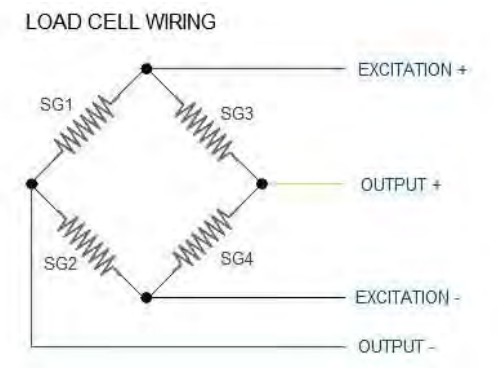
\includegraphics[width=0.3\textwidth]{./gambar/wheatstone_loadcell.png}
        \caption{Wheatstone Bridge Circuit on Load Cell\cite{rahman2018autonomous}.}
        \label{fig:Wheatstone_Bridge}
    \end{figure}
    
    \begin{equation}
      V_{\mathrm{out}} = V_{\mathrm{in}} \cdot \frac{R_2 \cdot R_3 - R_1 \cdot R_4}{(R_1 + R_2) \cdot (R_3 + R_4)}
      \label{eq:Wheatstone_Bridge}
    \end{equation}
    
    \hspace*{1em} In the Load Cell sensor, the system is equipped with a Wheatstone Bridge circuit. The Wheatstone Bridge, as shown in Figure \ref{fig:Wheatstone_Bridge}, is a circuit used to measure resistance changes with high sensitivity \cite{rahman2018autonomous}. To measure resistance changes, the Wheatstone Bridge equation is used as in Equation \ref{eq:Wheatstone_Bridge}.

    \item Real Time Operating System (RTOS)
    \label{subsec:rtos}

    \hspace*{1em} Real-Time Operating System (RTOS) is a crucial component in modern embedded systems. Its ability to manage concurrent tasks effectively allows the system to process data from various sensors, such as load cells, simultaneously, and control actuators with high precision \cite{sayyad2023real}. Timely task scheduling and efficient interrupt handling ensure quick and stable responses from the robot, which is essential in dynamic and complex robotic applications.

    \begin{figure} [h] \centering
      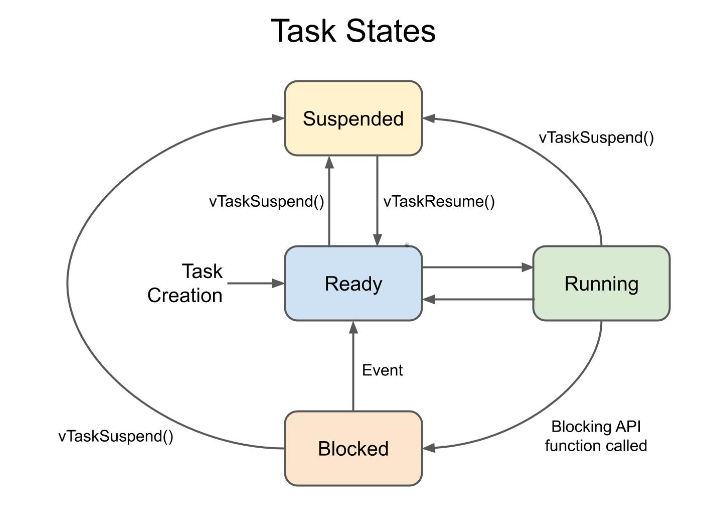
\includegraphics[scale=0.4]{gambar/rtos.png}
      \caption{Task Scheduling (RTOS)\cite{digikey2021task}.}
      \label{fig:RTOS}
    \end{figure}
  
    \hspace*{1em} The state diagram in Figure \ref{fig:RTOS} illustrates how RTOS allows the system to execute various tasks concurrently, prioritizing more critical tasks\cite{digikey2021task}. This enables the robot to respond quickly to environmental changes, such as maintaining balance, and overall improves the performance and adaptability of the robotic system.

    \item PID Control System
    \label{subsec:pidcontrolsystem}

    \hspace*{1em} The use of a PID (Proportional-Integral-Derivative) control system is a common method in servo motor control. This system helps maintain the balance and stability of the robot by correcting movements based on the error value generated from the difference between the actual position and the desired position. PID consists of three main components: proportional control (P), integral (I), and derivative (D). Each component functions to correct errors in different ways.

    \begin{equation}
      \mathrm{Correction} = K_p \cdot \mathrm{error} + K_i \cdot \int_{0}^{t} \mathrm{error} \cdot dt + K_d \cdot \frac{d\mathrm{error}}{dt}
    \end{equation}

    \hspace*{1em} The combination of these three components forms an effective PID control in maintaining the robot's balance and stability. Proper tuning of the $K_p$, $K_i$, and $K_d$ parameters is crucial to ensure optimal and responsive system performance.

    \item Center of Pressure
    \label{subsec:centerofpressure}

    \hspace*{1em} The center of pressure is the point where all forces are concentrated without any torque moment\cite{hawley2016external}. In this center of pressure, it consists of several pressures that are then calculated based on the cross-sectional area to determine the position of the center of pressure. The center of pressure is related to the robot's balance, particularly at the center of gravity\cite{arifin2017implementasi}.

    \begin{equation}
      X_{\mathrm{cop}} = X_0 + \frac{(F2 + F4) \cdot dx}{F1 + F2 + F3 + F4}
      \label{eq:COP_X_1}
    \end{equation}

    \begin{equation}
      Y_{\mathrm{cop}} = Y_0 + \frac{(F1 + F2) \cdot dy}{F1 + F2 + F3 + F4}
      \label{eq:COP_Y_1}
    \end{equation}

    \begin{figure} [h] \centering
      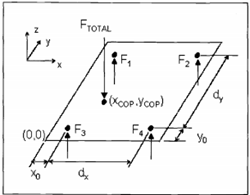
\includegraphics[width=0.3\textwidth]{gambar/Konsep_Letak.png}
      \caption{Concept of Center of Pressure Layout\cite{resna2005}.}
      \label{fig:Konsep_Letak}
    \end{figure}

    \hspace*{1em} Figure \ref{fig:Konsep_Letak} shows the concept of placing the pressure sensor. From this concept, the center of pressure can be calculated using Equation \ref{eq:COP_X_1} and Equation \ref{eq:COP_Y_1}.
\end{enumerate}
